\section{Introduction to Probabilities, Graphs, and Causal Models}

\begin{enumerate}
\item Bayesian interpretation of probability
\item Probabilities are degrees of belief
\item Beliefs are updated in response to observing data
\item E.g. $\p(H|e)$ is belief about hypothesis given evidence
  Alternatively: within the realities in which $E=e$, what is the distribution of $H$?
\item E.g. $\p(Y|x)$ is belief about outcome variable given treatment observed to be $X=x$
  Alternatively: within the cases in which $X=x$, what is the distribution of $Y$?
\item {\it independence}: $\forall x$ we have $\p(Y|x) = \p(Y)$
\end{enumerate}

Conditional probabilities are primitive; they are not defined in terms of joint probabilities. Instead
\begin{align*}
  \p(x, y) = \p(x)\p(y|x).
\end{align*}
Thus the law of total probability $\p(X) = \sum_Z\p(X, Z)$ gives rise to
\begin{align*}
  \p(y|x) = \sum_z \p(z)\p(y|x,z).
\end{align*}
This theorem lies behind the notion of ``controlling​'' for a covariate $Z$ when studying the effect of $X$ on $Y$.

\subsection{Bayes' rule}

Since conditional probabilities are primitive, Bayes' rule
\begin{align*}
  \p(H|e) = \p(H) \p(e|H) \times \p(e)^{-1}
\end{align*}
is a ``normative rule for updating beliefs in response to evidence​'', as opposed to a tautology (theorem) derivable from definitions of conditional probability.

\begin{quote}
  {\it Accordingly, (1.14) [Bayes' rule] is not a definition but rather an empirically verifiable relationship
    between English expressions.}
\end{quote}
\begin{question}
  What does that mean?
\end{question}

\begin{enumerate}
\item Belief in $h$ after observing $e$ increases (relative to $\p(h,e)$) in proportion to the degree of surprise of observing $e$.
\item Belief in $h$ after observing $e$ is never lower than prior belief in $(h, e)$.
\end{enumerate}

\begin{intuition}
  We're imagining possible pairs $(H, E)$ of explanation (hypothesis) and data (evidence) and have formed prior beliefs about their joint value. Then data $e$ becomes known. Belief about $h$ is now equal to $\p(h,e)$ multiplied by the surprise $\p(e)^{-1}$ of observing $e$.

  I'm not sure that's an interesting way of describing it really. I think I'd describe it as:
  \begin{enumerate}
  \item We have formed prior beliefs about $(H, E)$ pairs.
  \item We observe data.
  \item This causes all but one column of the joint distribution to be set to zero.
  \item To view the result as a probability distribution, we have to rescale (and drop a now-pointless dimension).
  \end{enumerate}
\end{intuition}


\subsection{Probability models, Boolean logic}

Given atomic propositions $A, B, C, \ldots$, a \defn{elementary event} is a conjunction involving the joint values of all of them, i.e. a sentence in which each proposition, or its negation, occurs exactly once, e.g.
\begin{align*}
  S = (A \land B) \lor \lnot C.
\end{align*}

\begin{theorem*}
  Elementary events are mutually exclusive and every boolean formula can be expressed as a disjunction of elementary events.
\end{theorem*}

The {\it sample space} of probability textbooks is (for discrete RVs) equivalent to the set of {\it elementary events} in propositional logic.

A \defn{probability model} gives the probability of every well-formed sentence. A joint probability distribution is a probability model.

\begin{quote}
  {\it In practice, however, joint distribution functions are rarely specified explicitly. In
    the analysis of continuous random variables, the distribution functions are given by
    algebraic expressions such as those describing normal or exponential distributions; for
    discrete variables, indirect representation methods have been developed where the overall
    distribution is inferred from local relationships among small groups of variables.
    Graphical models, the most popular of these representations, provide the basis of
    discussion throughout this book.}
\end{quote}

\begin{question}
  Is that saying graphical models apply only to discrete RVs??
\end{question}



\subsection{Odds, likelihood ratios}

The \defn{odds} of $H$ are a measure of strength of belief in $H$:
\begin{align*}
  O(H) = \frac{\p(H)}{\p(\lnot H)} = \frac{\p(H)}{1 - \p(H)}.
\end{align*}
Bayes' rule says that
\begin{align*}
 \p(H|e) = \p(H) \p(e|H) \times \p(e)^{-1},
\end{align*}
therefore the posterior strength of belief in $H$ is equal to the prior strength of belief, multiplied by the likelihood ratio:
\begin{align*}
  O(H|e) = O(H) \times \frac{\p(e|H)}{~\p(e|\lnot H)}.
\end{align*}

\subsection{Expected values}

\begin{tabular}{l l l}
Expectation                  & $\E[f(x)] = \sum_x f(x) \p(x)$                                                & centroid \\
Variance                       & $\Var[Z] = \sigma^2_Z = \E\Big[(Z - \E[Z])^2\Big]$                     & average distance (squared) from center in 1D \\
Covariance                    & $\Cov[X, Y] = \sigma_{XY} = \E\Big[(X - \E[X])(Y - \E[Y])\Big]$   & average size of squares from center in 2D \\
Correlation coefficient     & $\rho_{XY} = \sigma_{XY} / \sigma_X\sigma_Y$                             & average size of squares from center in 2D, scaled by both variances\\
Regression coefficient      & $r_{XY} = \sigma_{XY} / \sigma^2_{Y}$                                      & average size of squares from center in 2D, scaled by one variance
\end{tabular}

\subsection{Conditional independence and graphoids}

Let $W_1, W_2, \ldots, X_1, X_2, \ldots, Y_1, Y_2, \ldots, Z_1, Z_2, \ldots$ be random variables with some
joint distribution.

Let $W, X, Y, Z$ be subsets of these random variables, so that for example $W = \{W_1, W_2, \ldots \}$.

\begin{definition}[Conditional independence of sets of random variables]
  We write $(X \indep Y ~|~ Z)$ to mean that
\begin{align*}
  \p(X_i=x ~|~ Y_j=y, Z_k=z) = \p(X_i=x ~|~ Z_k=z)
\end{align*}
for all $x$, $y$, $z$, and for all valid values of the indices $i$, $j$, $k$.

We say that the set $X$ is independent of the set $Y$ given the set $Z$.
\end{definition}

\begin{definition}[Product]
  \begin{align*}
    YW = \Big\{(Y_i, W_j) ~\Big|~ i \in \{1, \ldots, n_Y,\}, j \in \{1, \ldots, n_W\}\Big\}.
  \end{align*}
\end{definition}

\begin{theorem}[Weak union]
  \begin{align*}
    (X \indep YW ~|~ Z) \implies (X \indep Y | WZ).
  \end{align*}
    In other words, if
    \begin{align*}
      \p(X_i=x ~|~ (YW)_j=u, Z_k=z) = \p(X_i=x ~|~ Z_k=z)
    \end{align*}
    for all $i, j, k$, then
    \begin{align*}
      \p(X_i=x ~|~ Y_j=y, (WZ)_k=v) = \p(X_i=x ~|~ (WZ)_k=v)
    \end{align*}
    for all $i, j, k$.
\end{theorem}






\begin{proof}
  Suppose that
    \begin{align*}
      \p(X_i=x ~|~ (YW)_j=u, Z_k=z) = \p(X_i=x ~|~ Z_k=z)
    \end{align*}
    for all $i, j, k$.

    Written without the product notation, this statement is
    \begin{align*}
      \p(X_i=x ~|~ Y_j=y, W_k=w, Z_l=z) = \p(X_i=x ~|~ Z_l=z)
    \end{align*}
    for all $i, j, k, l$.

    This is equivalent to
    \begin{align*}
      \p(X_i=x ~|~ Y_j=y, (WZ)_k=v) = \p(X_i=x ~|~ Z_l=z)
    \end{align*}
    for all $i, j, k$.

    We want to show that
    \begin{align*}
      \p(X_i=x ~|~ Y_j=y, (WZ)_k=v) = \p(X_i=x ~|~ (WZ)_k=v)
    \end{align*}
    or equivalently that
    \begin{align*}
      \p(X_i=x ~|~ Z_l=z)  = \p(X_i=x ~|~ (WZ)_k=v)
    \end{align*}


\end{proof}


  In other words, let
  \begin{align*}
  \p(X_i=x ~|~ Y_j=y, W_k=w, Z_l=z) = \p(X_i=x ~|~ Z_l=z)
  \end{align*}
  for all valid values of the indices $i, j, k, l$.

  Then
  \begin{align*}
    \p(X_i=x|Y_j=y, W_k=w, Z_l=z) = \p(X_i=x|Z_l=z, W_k=w).
  \end{align*}

We write the Weak union implication as
  \begin{align*}
    (X \indep YW ~|~ Z) \implies (X \indep Y | ZW).
  \end{align*}









 This implies the conditional independence of all pairs of component variables,
but the converse is not necessarily true. $Z$ may be empty in which case the statement is that $X \indep Y$.

Conditional independence between subsets obeys some fairly unsurprising laws:

\begin{itemize}
  \begin{table}[!h]
    \centering
    \begin{tabular}{|l|l l l l}
      {\bf Symmetry}      & $X \indep Y  ~|~ Z $&$                            $&$\implies Y \indep X  ~|~ Z   $ & \\
      {\bf Decomposition} & $X \indep YW ~|~ Z $&$                           $&$\implies X \indep Y  ~|~ Z   $ &\\
      {\bf Weak union}    & $X \indep YW ~|~ Z $&$                           $&$\implies X \indep Y  ~|~ ZW  $ &\\
      {\bf Contraction}   & $X \indep Y  ~|~ Z  $&$ ~~\&~~ X \indep W ~|~ ZY  $&$\implies X \indep YW ~|~ Z   $ & \\
      {\bf Intersection}  & $X \indep W  ~|~ ZY $&$ ~~\&~~ X \indep Y ~|~ ZW  $&$\implies X \indep WY ~|~ Z   $ &
  \end{tabular}
    \caption{Properties of conditional independence relation between subsets}
  \end{table}
\end{itemize}

\begin{itemize}
\item Graph >
\item Directed Graph >
\item Directed Acyclic Graph >
\item Tree (nodes have one or zero parents)
\end{itemize}

\begin{definition}[Parent]
\defn{Parents} $PA_j$ are a minimal set of ancestors such that, conditional on knowing their values, all other
values are irrelevant to the probability distribution at node $j$.
\end{definition}

\begin{definition}[Markov Compatability]
  A joint probability distribution $P$ is \defn{compatible} with a graph $G$ if $P$ factorizes according to the
  parent relationships of $G$. I.e.
\begin{align*}
  P(x_1, x_2, \ldots) = \prod_i P(x_i|pa_i)
\end{align*}
 Synonyms:
 \begin{itemize}
 \item $G$ \defn{represents} $P$
 \item $P$ is \defn{Markov} relative to $G$
 \end{itemize}
\end{definition}

\begin{definition}[$d$-Separation, ``blocked​'']
  A set of nodes $Z$ \defn{blocks} $X$ from $Y$ if for every path between a node in $X$ and a node in $Y$ one
  of the following is true (i.e. the path is ``blocked​''):
  \begin{itemize}
  \item The path contains a chain $i \rightarrow m \rightarrow k$ or a fork $i \leftarrow m \rightarrow k$ with the middle node $m$ in $Z$.
  \item The path contains a collider $i \rightarrow m \leftarrow k$ with $m$ not in $Z$ and no descendent of $m$ in $Z$.
  \end{itemize}
\end{definition}

\begin{intuition}
  Let the arrows denote causality and suppose $Z$ represents observed nodes.
  \begin{itemize}
  \item The first condition is saying that $i$ and $j$ are independent because we have observed the middle node
    that was mediating their causal connection (dependence).
  \item The second condition is saying $i$ and $j$ are independent because we have not observed the middle node
    that would be inducing dependence were it observed.
  \end{itemize}
\end{intuition}




Here, $Z$ $d$-separates $X$ and $Y$. Intuitively, $Z$ represents a set of observed nodes. $x_1$ and $y_1$
are independent because $z_1$ is observed, and $x_2$ and $y_2$ are independent because $m_2$ is not observed.

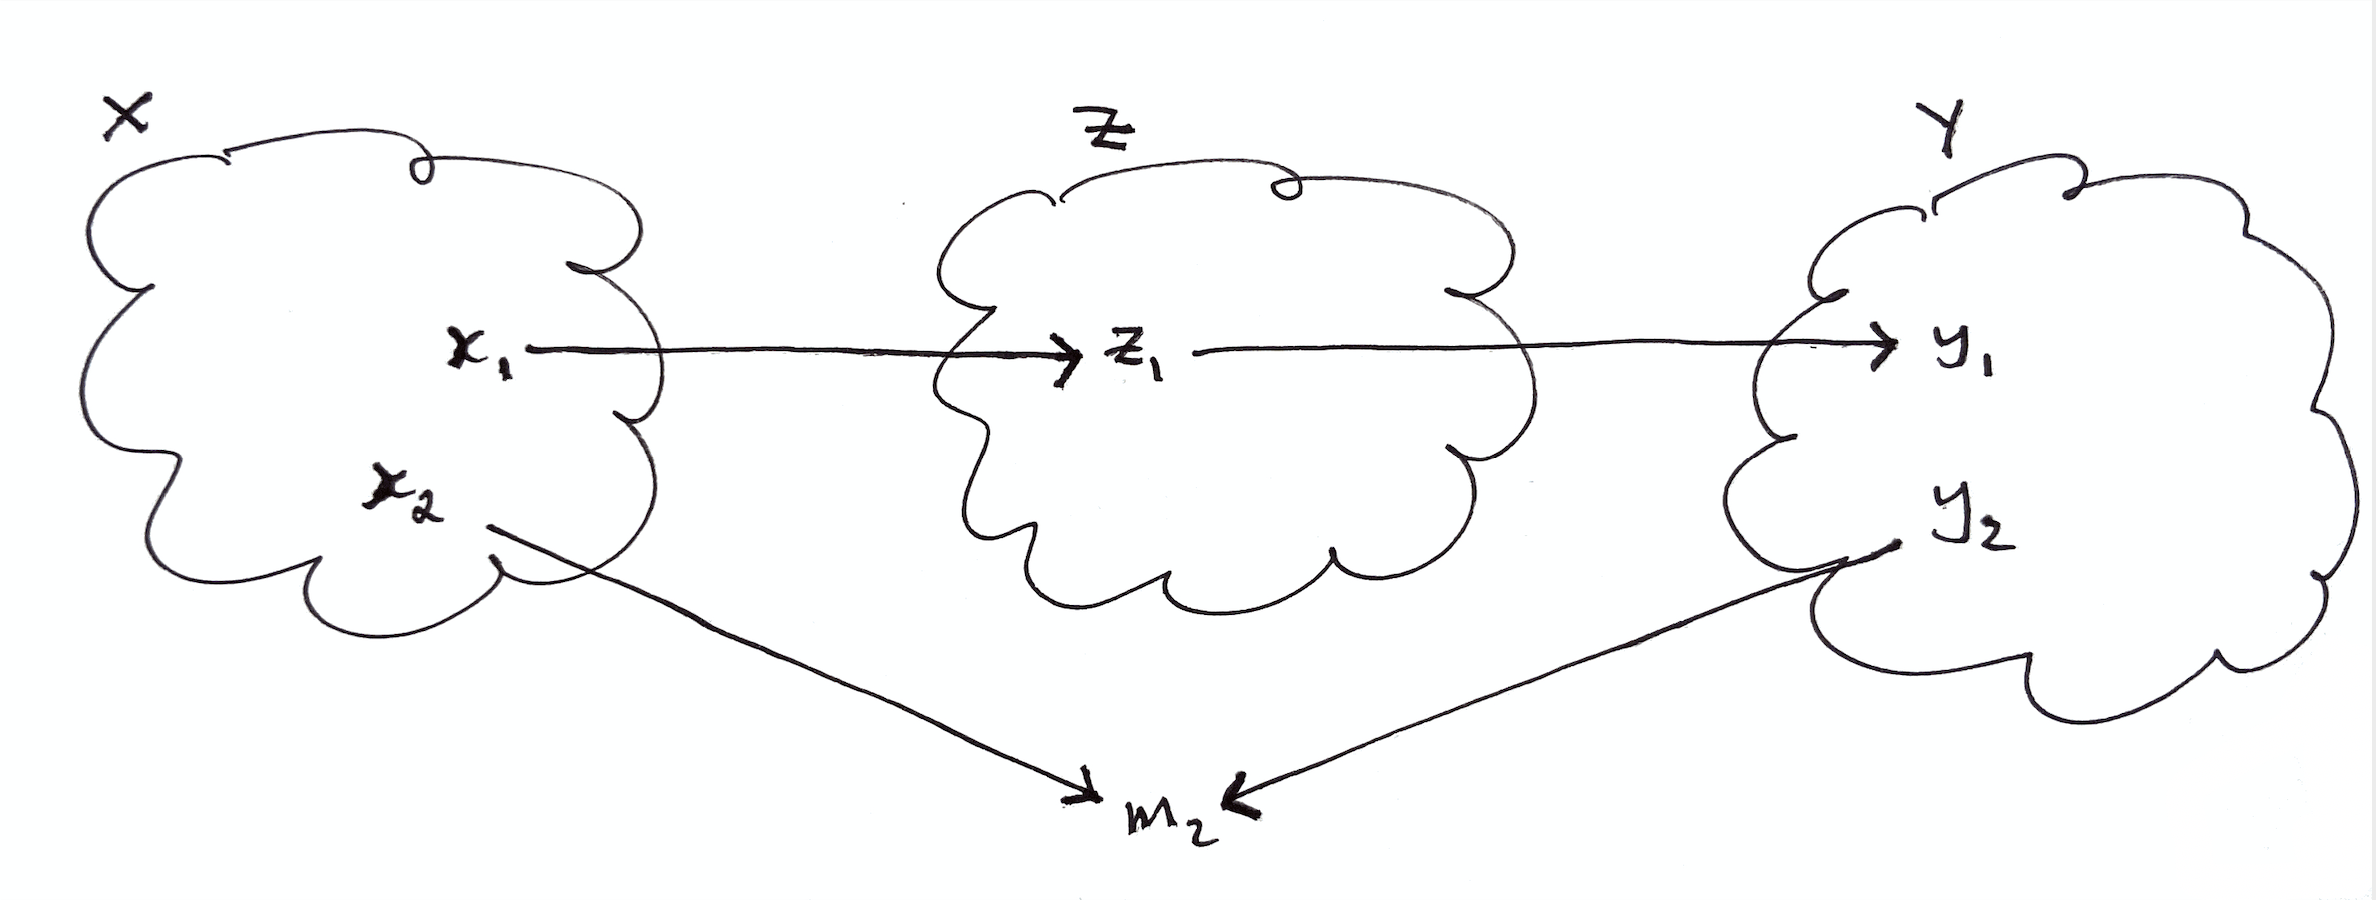
\includegraphics[width=400pt]{img/statistics-and-machine-learning--pearl--causality--conditional-independence-and-graphoids-1231.png}

But why isn't this a counter-example? Although $m_2$ is still unobserved, we have information about it because
it is dependent on $z_2$, which is observed.

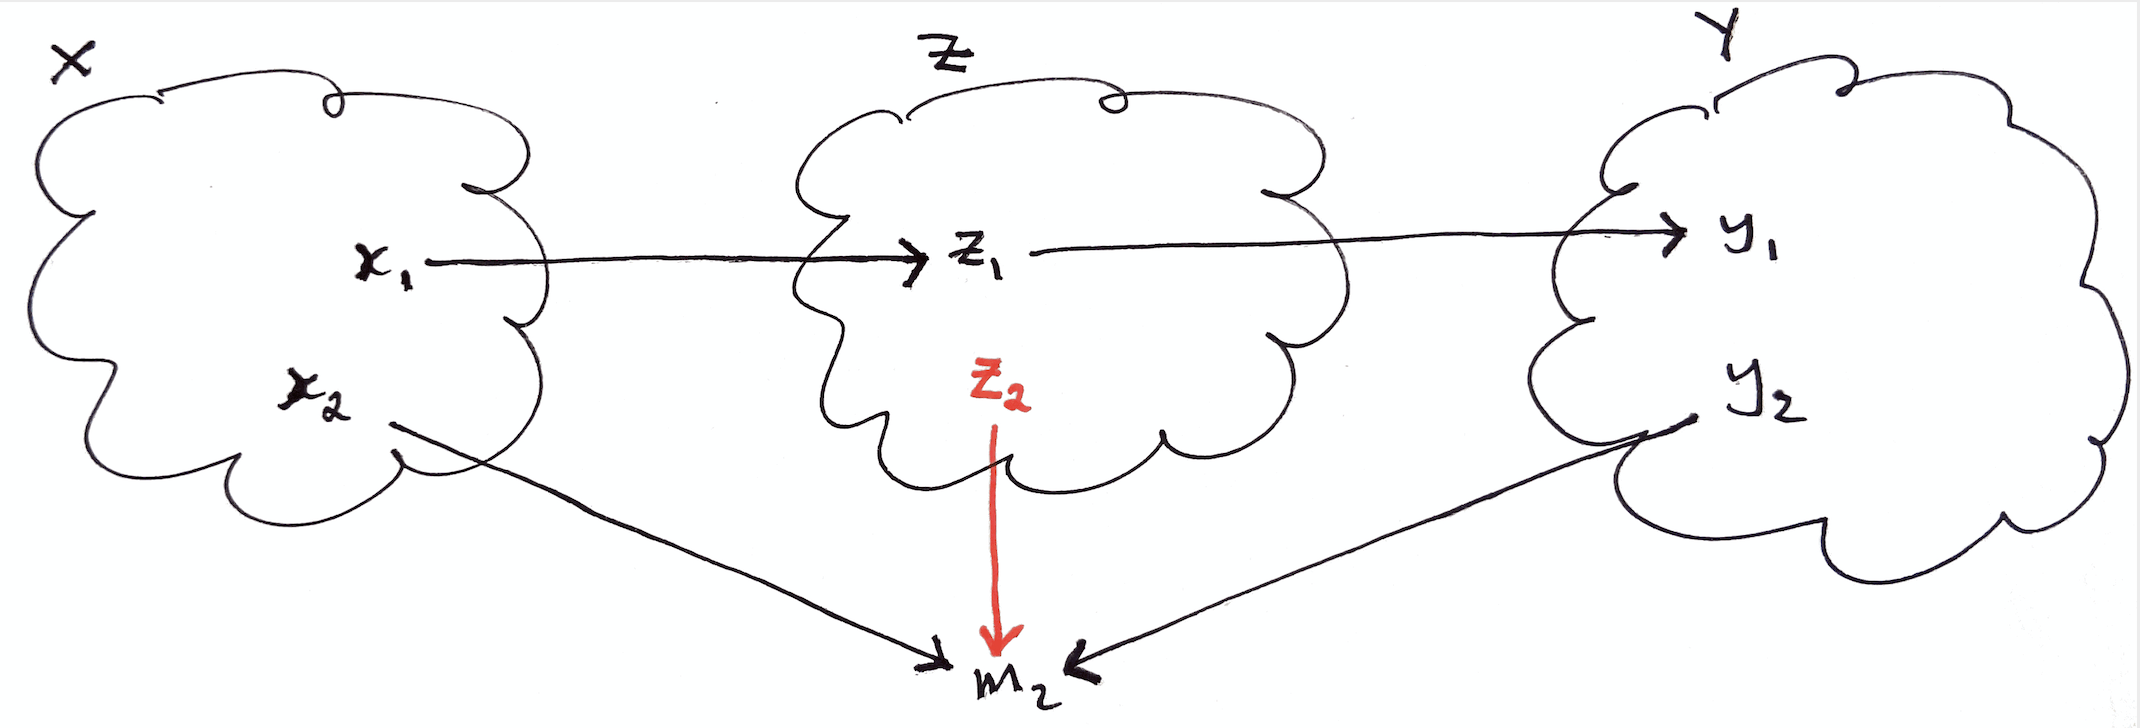
\includegraphics[width=400pt]{img/statistics-and-machine-learning--pearl--causality--conditional-independence-and-graphoids-7e5e.png}

The graphical condition of $d$-separation implies theorems about probability distributions that are compatible with the graph. E.g.

\begin{theorem}[$d$-Separation and probability distributions]
  If $X$ and $Y$ are $d$-separated by $Z$ in graph $G$, then $X \indep Y ~|~ Z$ in every probability
  distribution compatible with $G$.

  Conversely, if they are not $d$-separated, then there exists a probability distribution compatible with $G$
  in which they are not conditionally independent. (In fact, they are conditionally dependent in ``almost all​''
  probability distributions compatible with $G$.)
\end{theorem}

\begin{definition}[Skeleton]
  The \defn{skeleton} of a directed graph $G$ is the graph that results on converting all directed edges into
  undirected edges.
\end{definition}

\begin{definition}[Observational Equivalence]
  TODO
\end{definition}

\begin{theorem}[Observational Equivalence]
  Two DAGs are observationally equivalent if they have the same skeleton and the same set of {\it v-structures} (two
  convergent arrows whose tails are not joined by an arrow).
\end{theorem}

https://arxiv.org/pdf/1304.1108.pdf

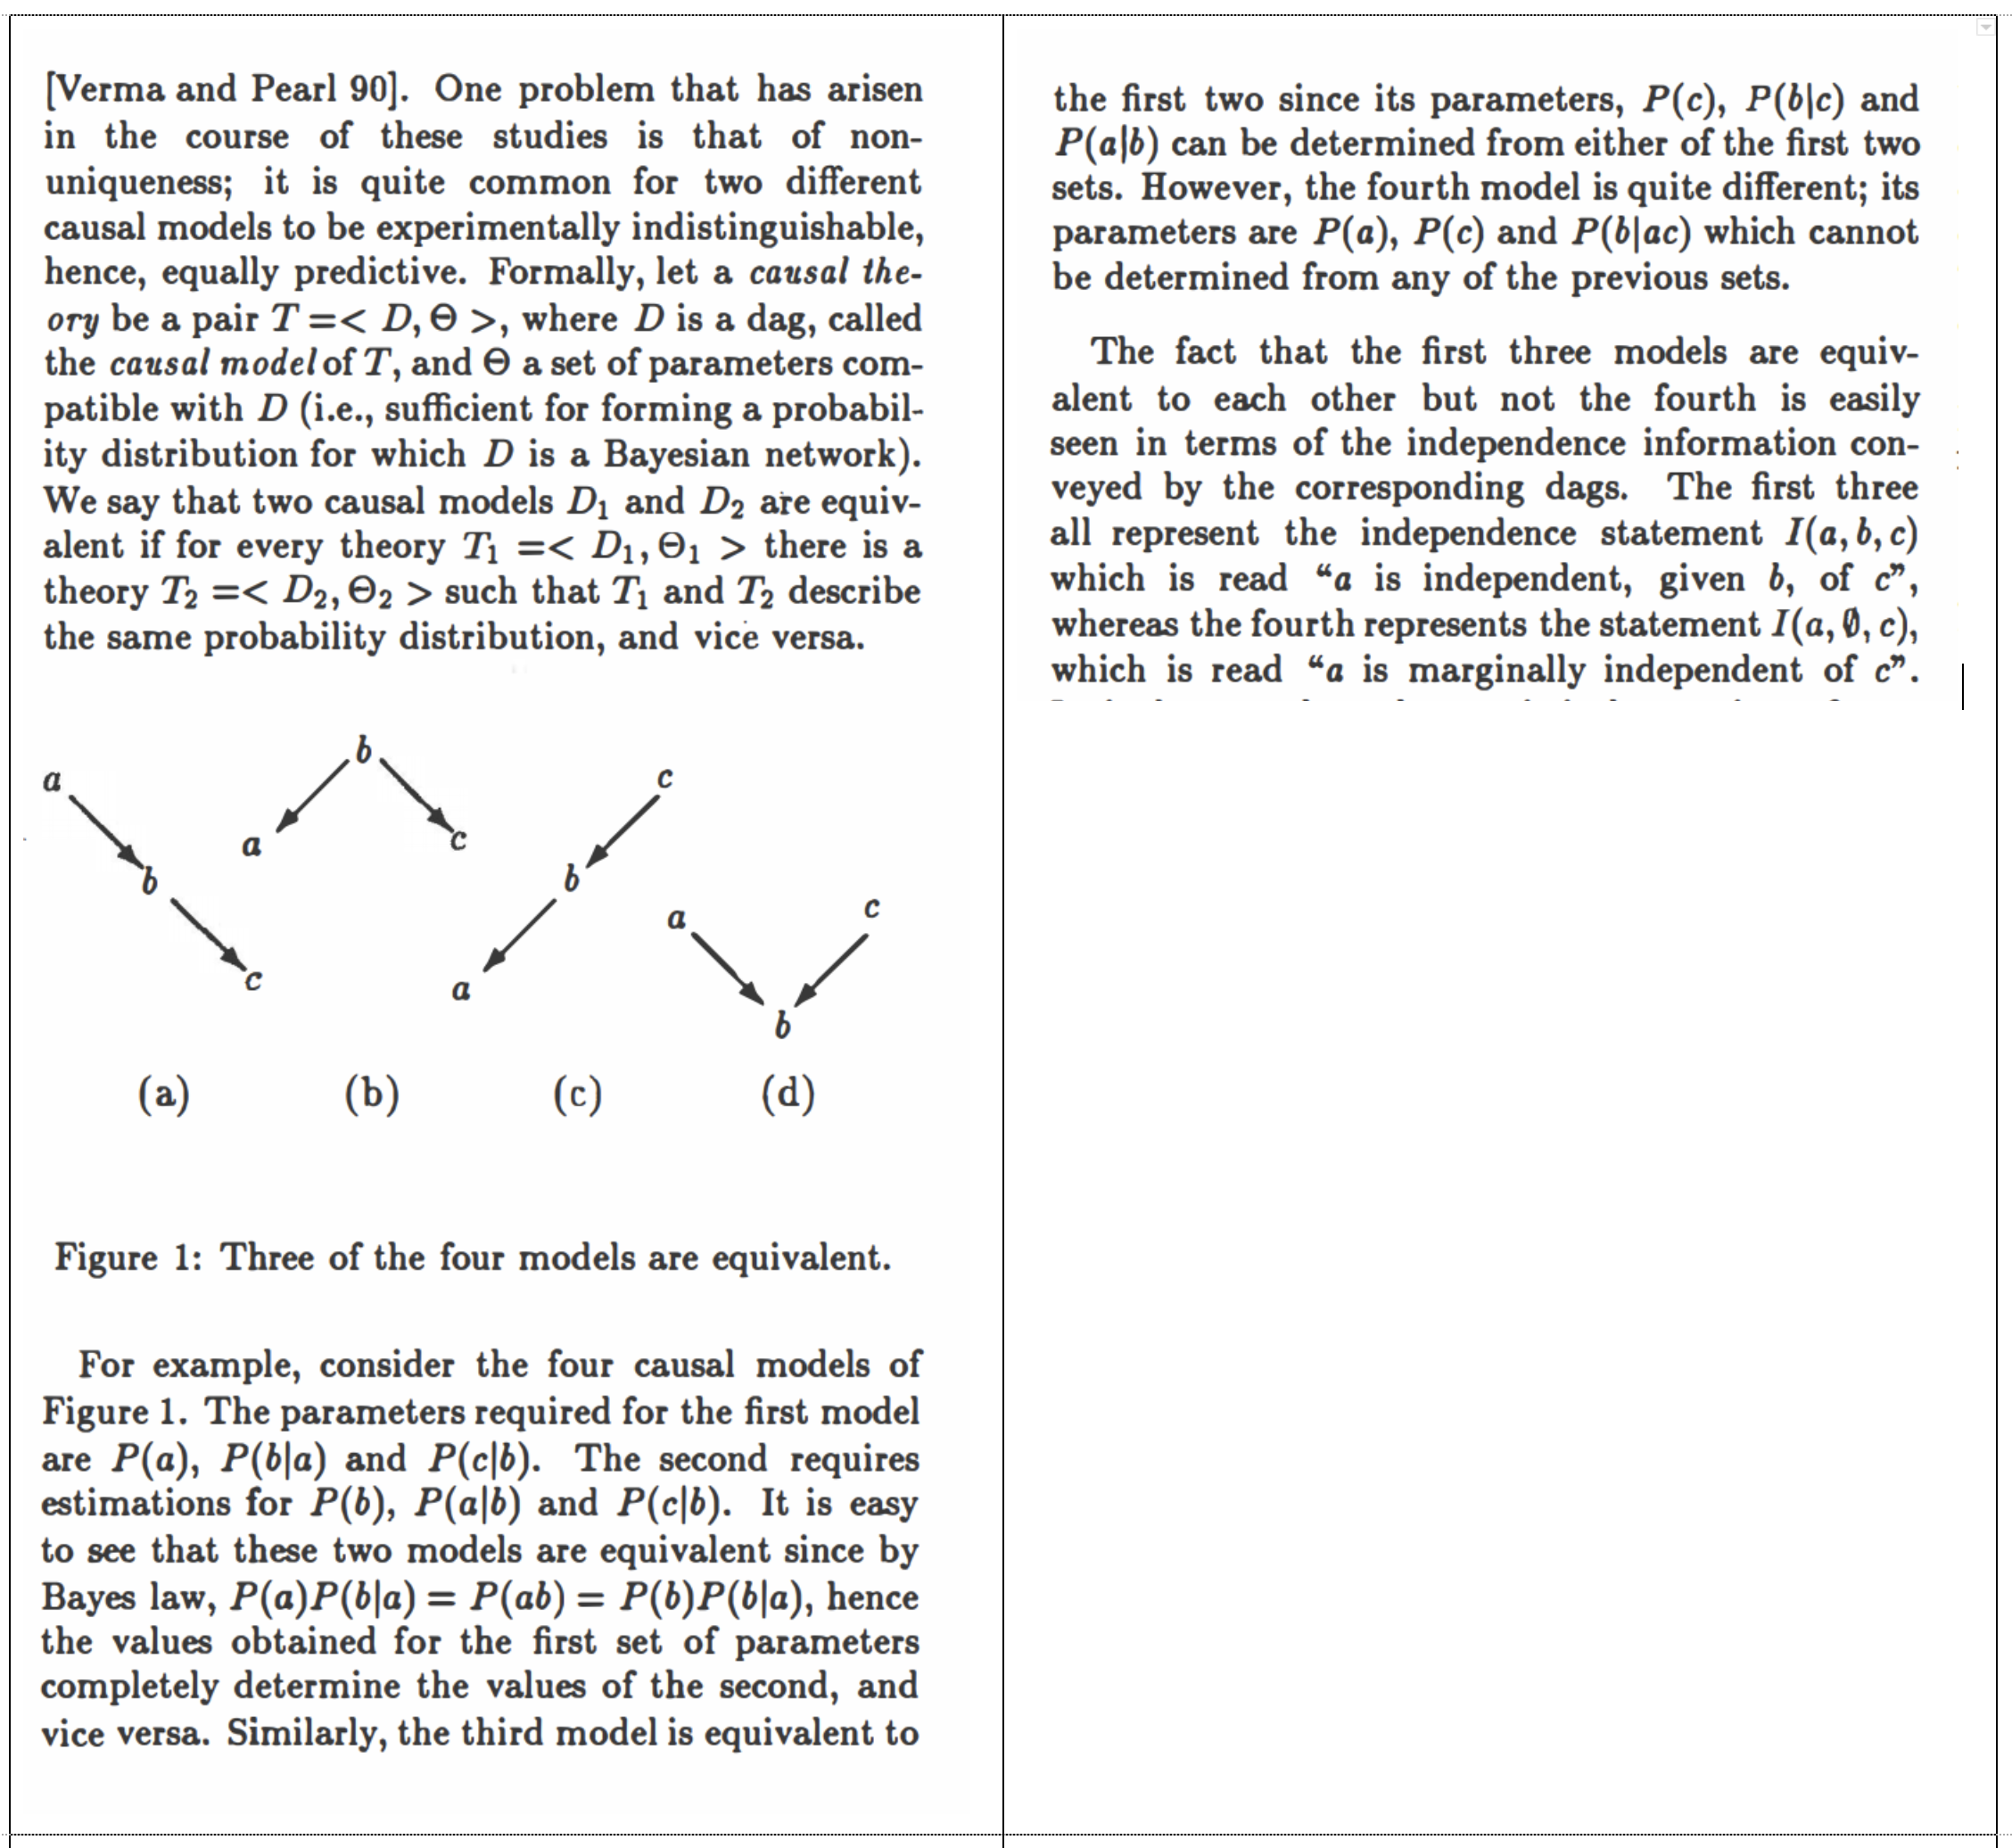
\includegraphics[width=400pt]{img/statistics-and-machine-learning--pearl--conditional-independence-and-graphoids-39eb.png}


\begin{intuition}
  \begin{itemize}
  \item If we define data to be ``stuff that is spat out by a probability distribution​'', then we can only use data
    to distinguish two explanations if the explanations involve different probability distributions.
  \item For a DAG $G$, there are many compatible probability distributions.
  \item For a probability distribution $P$, there are multiple compatible DAGs.
  \item For example, consider $P(A, B)$.
  \end{itemize}
\end{intuition}

In other words, consider the possible joint distributions over $(A, B, C)$. the following factorizations/DAGs
are all observationally equivalent. They make the conditional independence asssertions that: TODO

\begin{table}[!h]
  \centering
  \begin{tabular}{|c|c|}
    Factorization & DAG \\
    \hline&\\
    $\p(A)\p(B|A)\p(C|B)$&\adjustbox{valign=m}{\begin{tikzpicture}\graph{A -> B -> C};\end{tikzpicture}}\\
    &\\\hline&\\
    $\p(C)\p(B|C)\p(A|B)$&\adjustbox{valign=m}{\begin{tikzpicture}\graph{A <- B <- C};\end{tikzpicture}}\\
    &\\\hline&\\
    $\p(B)\p(A|B)\p(C|B)$&\adjustbox{valign=m}{\begin{tikzpicture}\graph{B -> A, B -> C};\end{tikzpicture}}\\
    &\\\hline&\\
  \end{tabular}
\end{table}

But this one is not observationally equivalent to those. The conditional independence assertions that it makes are: TODO

\begin{table}[!h]
  \centering
  \begin{tabular}{|c|c|}
    Factorization & DAG \\
    \hline&\\
    $\p(A)\p(C)\p(B|A,C)$&\adjustbox{valign=m}{\begin{tikzpicture}\graph{A -> B, B <- C};\end{tikzpicture}}\\
    &\\\hline&\\
  \end{tabular}
\end{table}
What about this one?

\begin{table}[!h]
  \centering
  \begin{tabular}{|c|c|}
    Factorization & DAG \\
    \hline&\\
    $\p(A)\p(B)  \p(C|B)$&\adjustbox{valign=m}{\begin{tikzpicture}\graph{A, B -> C};\end{tikzpicture}}\\
    &\\\hline&\\
  \end{tabular}
\end{table}

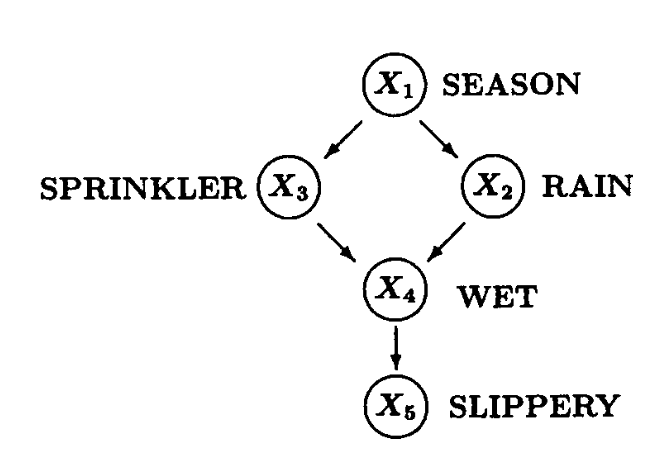
\includegraphics[width=200pt]{img/statistics-and-machine-learning--pearl--causality--conditional-independence-and-graphoids-cddf.png}

\begin{quote}
  It seems that if conditional independence judgments are by-products of stored causal relationships, then
  tapping and representing those relationships directly would be a more natural and more reliable way of
  expressing what we know or believe about the world. This is indeed the philosophy behind causal Bayesian
  networks.
\end{quote}
